\subsection{M.PC.AC - Actual Cost}
\label{sec:AC}

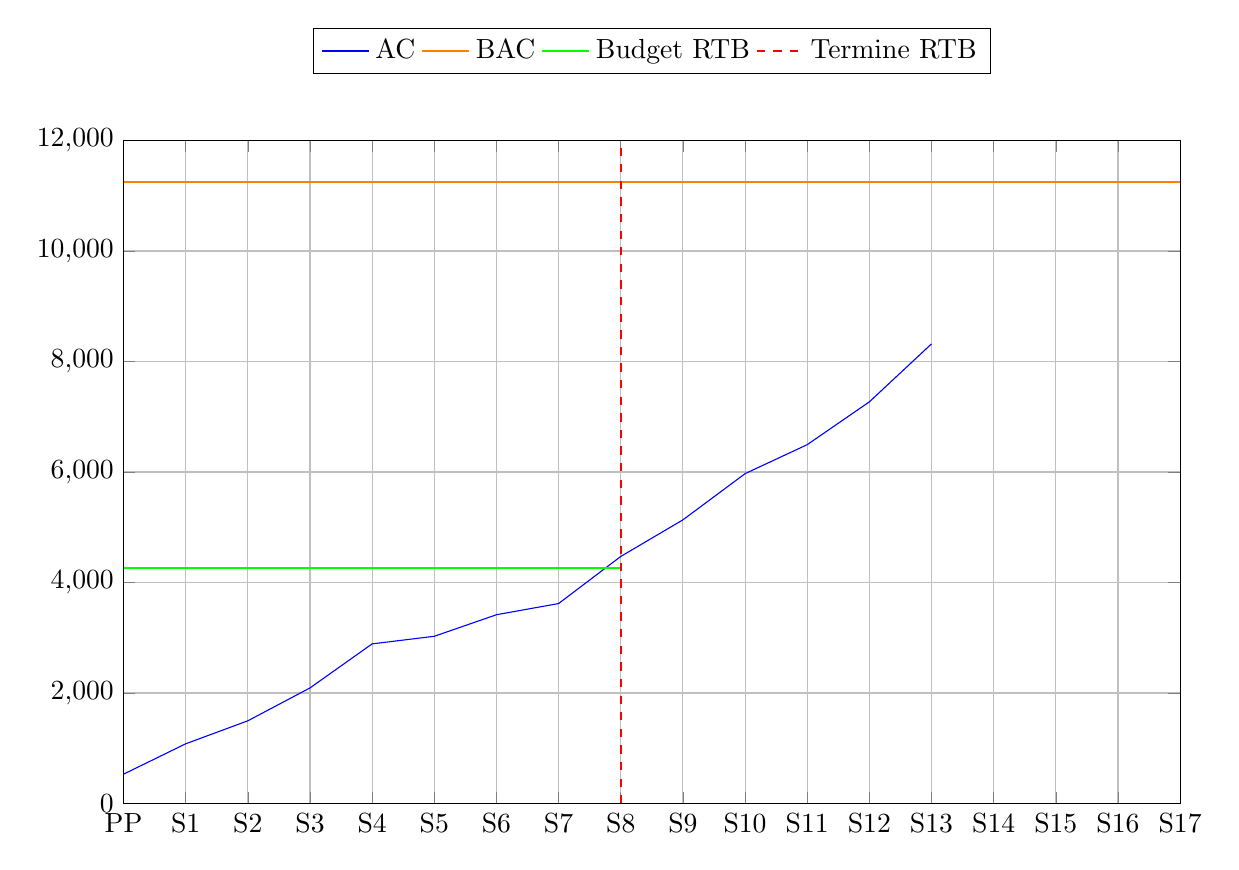
\begin{tikzpicture}
    \begin{axis}[
        width=15cm, height=10cm,
        ymin=0, ymax=12000,
        xmin=0, xmax=17,
        xtick={0, 1, 2, 3, 4, 5, 6, 7, 8, 9, 10, 11, 12, 13, 14, 15, 16, 17, 18},
        xticklabels={PP, S1, S2, S3, S4, S5, S6, S7, S8, S9, S10, S11, S12, S13, S14, S15, S16, S17, S18},
        xlabel={},
        ylabel={},
        grid=major,
        scaled ticks=false,
        legend style={at={(0.5,1.1)}, anchor=south, legend columns=-1},
    ]
    \addplot[color=blue] coordinates {(0, 530) (1, 1080) (2, 1496.25) (3, 2091.25) (4, 2888.75) (5, 3026.25) (6, 3416.25) (7, 3618.75) (8, 4471.25) (9, 5133.75) (10, 5970) (11, 6495) (12, 7270) (13, 8320)};
    \addlegendentry{AC}
    \addplot[orange, thick] coordinates {(0, 11250) (17, 11250)};
    \addlegendentry{BAC}
    \addplot[green, thick] coordinates {(0, 4265) (8, 4265)};
    \addlegendentry{Budget RTB}
    \addplot[red, thick, dashed] coordinates {(8, 0) (8, 12000)};
    \addlegendentry{Termine RTB}
    \end{axis}
\end{tikzpicture}
\subsubsection{RTB}
Il grafico mostra l'incremento progressivo dei costi totali sostenuti a ogni \glossario{sprint}, 
includendo sia i costi per le attività completate sia quelli per le attività ancora in corso.

\paragraph{Sprint 9}
Il costo totale sostenuto è di 5133.75 euro, che corrisponde a circa il 45.7\% del budget totale previsto per il progetto.

\paragraph{Sprint 10}
Il costo totale sostenuto è di 5970 euro, che corrisponde a circa il 53.06\% del budget totale previsto per il progetto.

\paragraph{Sprint 11}
Il costo totale sostenuto è di 6495 euro, che corrisponde a circa il 57.73\% del budget totale previsto per il progetto.

\paragraph{Sprint 12}
Il costo totale sostenuto è di 7270 euro, che corrisponde a circa il 64.6\% del budget totale previsto per il progetto.

\paragraph{Sprint 13}
Il costo totale sostenuto è di 8320 euro, che corrisponde a circa il 74\% del budget totale previsto per il progetto.
